% Evaluation criterion:
%- Language and use of figures
%- Clarity of the problem statement
%- Overall document structure
%- Depth of understanding for the field of computer architecture
%- Depth of understanding of the investigated problem

\section{Result}
\label{sec:result}

The speedup from running the selected applications with the different
prefetchers is tabulated in \autoref{fig:initResults}. The number of
prefetches issued by each algorithm is shown in
\autoref{tab:numPrefetches}.
% These speedups are calculated from stats from m5... Don't need this
% here, have already written this in methodology/intro - right?

\begin{figure}[ht]
  \centering
  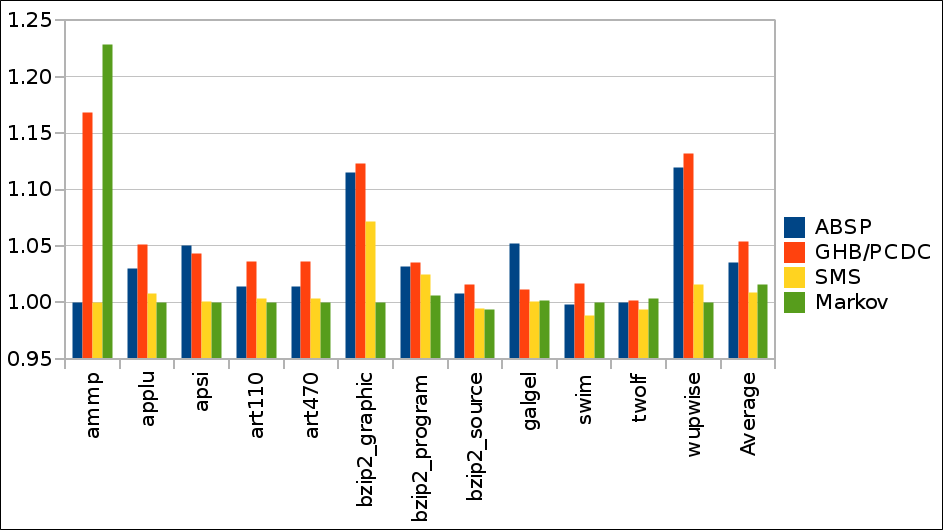
\includegraphics[scale=0.25]{figures/init_results.png}
  \caption{\label{fig:initResults} Speedup on the Y-axis plotted
    against program on the X-axis. The average values are calculated
    with a harmonic mean.}
\end{figure}

\begin{table}[htbp]
  \centering
  \begin{tabular}{|c|c|c|c|c|}
    \hline
    \textbf{Program} & \textbf{ABSP} & \textbf{GHB/PCDC} & \textbf{SMS} & \textbf{Markov} \\ \hline
    ammp             & 7             & 11133102          & 2629         & 7359044 \\ \hline
    applu            & 181817        & 1031986           & 63999        & 214880 \\ \hline
    apsi             & 52894         & 60416             & 879          & 7473 \\ \hline
    art110           & 1205703       & 2987084           & 325551       & 1623008 \\ \hline
    art470           & 1205703       & 2987084           & 325551       & 1623008 \\ \hline
    bzip2\_graphic   & 52339         & 64649             & 45194        & 697 \\ \hline
    bzip2\_program   & 16802         & 31978             & 19994        & 935 \\ \hline
    bzip2\_source    & 16124         & 22196             & 10391        & 503 \\ \hline
    galgel           & 171849        & 434138            & 37906        & 21337 \\ \hline
    swim             & 10263         & 1487464           & 287655       & 101607 \\ \hline
    twolf            & 41            & 54773             & 115217       & 236883 \\ \hline
    wupwise          & 308489        & 332550            & 61077        & 43555 \\ \hline
  \end{tabular}
  \caption{The number of memory addresses prefetched on each benchmark by each prefetcher.}
  \label{tab:numPrefetches}
\end{table}


Detailed data of the results from the optimal parameter search as
described in \autoref{sec:methodology} is not included, being just an
intermediate step towards performing a just comparison of the
different prefetchers.

%What other results? Should we include parameter search results? What
%about results from experimenting with altering the prefetchers---does
%that belong here or in the discussion section?XS
%
%\subsection{Sequential Prefetcher Result}
%\label{sec:sequentialPrefetcherResult}
%
%\subsection{GHB Prefetcher Result}
%\label{sec:ghbPrefetcherResult}
%
%\subsection{Markov Prefetcher Result}
%\label{sec:markovPrefetcherResult}
%
%\subsection{Spatial Memory Streaming Prefetcher Result}
%\label{sec:smsPrefetcherResult}

